\documentclass[tikz, border=10pt]{standalone}
\usetikzlibrary{positioning, arrows.meta}

\begin{document}
	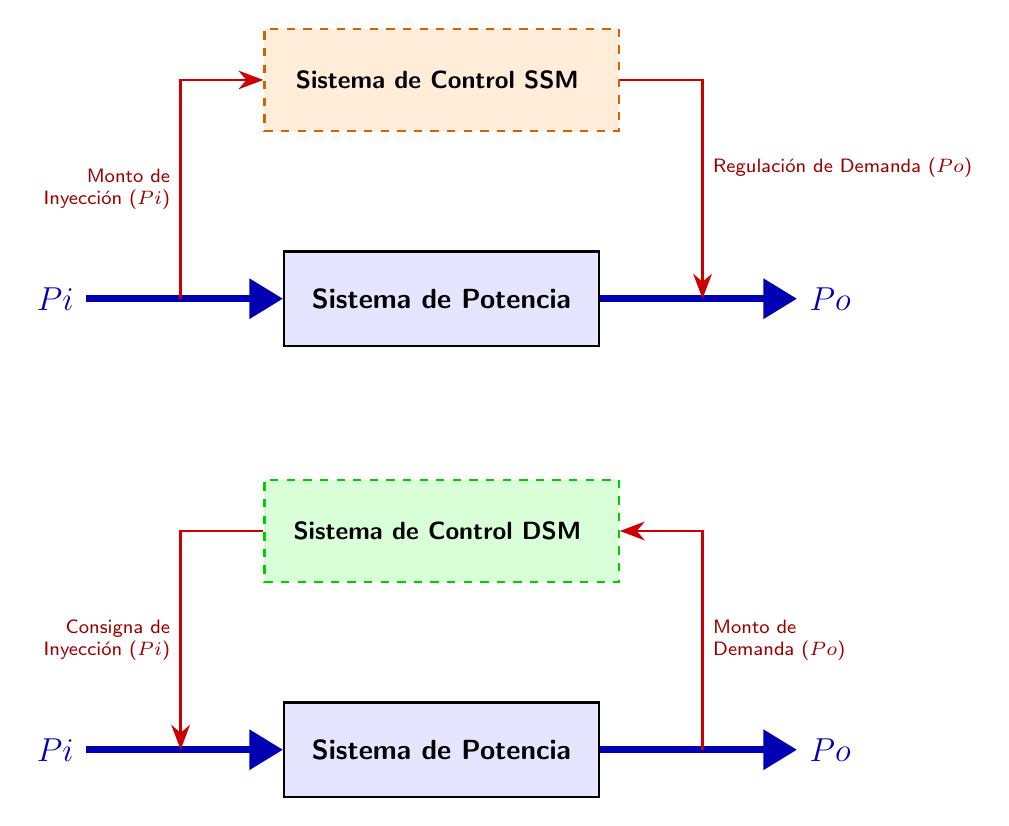
\begin{tikzpicture}[
		% --- ESTILOS DE BLOQUES ---
		planta/.style={
			rectangle, draw=black, fill=blue!10, thick,
			minimum width=4cm, minimum height=1.2cm, align=center,
			font=\sffamily\bfseries
		},
		control/.style={
			rectangle, draw=black, dashed, thick,
			minimum width=4.5cm, minimum height=1.3cm, align=center,
			font=\sffamily\small
		},
		% --- ESTILOS DE FLECHAS ---
		potencia/.style={
			-{Triangle[scale=1.2]}, line width=2.5pt, draw=blue!70!black
		},
		informacion/.style={
			-{Stealth[scale=1.2]}, line width=1pt, draw=red!80!black
		},
		% --- ESTILOS DE TEXTO ---
		etiqueta/.style={
			font=\sffamily\bfseries\large, color=blue!70!black
		},
		num/.style={
			font=\sffamily\color{gray!80!black}\tiny
		}
		]
		
		    % =========================================================================
		% BLOQUE 1: SISTEMA DE POTENCIA CON CONTROL SSM (Corregido y verificado)
		% =========================================================================
		
		\node[planta] (planta1) {Sistema de Potencia};
		%\node[num, above left=0.1cm and 0.1cm of planta1] {(1)};
		
		% Flujos de Potencia (Líneas físicas horizontales en y=0)
		\draw[potencia] (planta1.west) ++(-2.5cm,0) coordinate (p1in) -- (planta1.west) 
		node[pos=0.0, left, etiqueta] {$Pi$};
		
		\draw[potencia] (planta1.east) -- ++(2.5cm,0) coordinate (p1out) 
		node[pos=1.0, right, etiqueta] {$Po$};
		
		% Controlador SSM (Ubicado arriba de la planta)
		\node[control, above=1.5cm of planta1, fill=orange!15, draw=orange!80!black] (ssm) {
			\textbf{Sistema de Control SSM}
		};
		
		% LÓGICA DE CONTROL SSM EN DETALLE:
		
		% 1. Entrada (Izquierda): Sube desde el flujo Pi hacia el lado izquierdo del SSM
		\draw[informacion] ([xshift=1.2cm]p1in) |- (ssm.west)
		node[pos=0.25, left, font=\sffamily\scriptsize\color{red!60!black}, align=right] {Monto de\\Inyección ($Pi$)};
		
		% 2. Salida (Derecha/Izquierda): Nace en ssm.west, va a la izquierda, cruza por arriba 
		%    y BAJA apuntando verticalmente hacia abajo sobre el flujo Po (derecha)
		\draw[informacion] (ssm.east) -- ++(0,0)  -| ([xshift=-1.2cm]p1out)
		node[pos=0.7, right, font=\sffamily\scriptsize\color{red!60!black}] {Regulación de Demanda ($Po$)};
		
		% =========================================================================
		% BLOQUE 2: SISTEMA DE POTENCIA CON CONTROL DSM (Mide Po -> Modula Pi)
		% =========================================================================
		
		\node[planta, below=4.5cm of planta1] (planta2) {Sistema de Potencia};
%		\node[num, above left=0.1cm and 0.1cm of planta2] {(2)};
		
		% Flujos de Potencia (Líneas físicas horizontales)
		\draw[potencia] (planta2.west) ++(-2.5cm,0) coordinate (p2in) -- (planta2.west) 
		node[pos=0.0, left, etiqueta] {$Pi$};
		
		\draw[potencia] (planta2.east) -- ++(2.5cm,0) coordinate (p2out) 
		node[pos=1.0, right, etiqueta] {$Po$};
		
		% Controlador DSM
		\node[control, above=1.5cm of planta2, fill=green!15, draw=green!80!black] (dsm) {
			\textbf{Sistema de Control DSM}
		};
		
		% LÓGICA DE CONTROL DSM:
		% 1. El DSM recibe información del monto Po (Demanda)
		\draw[informacion] (p2out) ++(-1.2cm, 0) |- (dsm.east)
		node[pos=0.25, right, font=\sffamily\scriptsize\color{red!60!black}, align=left] {Monto de\\Demanda ($Po$)};
		
		% 2. El DSM emite información para regular el monto Pi (Inyección)
		\draw[informacion] (dsm.west) -| ([xshift=1.2cm]p2in)
		node[pos=0.75, left, font=\sffamily\scriptsize\color{red!60!black}, align=right] {Consigna de\\Inyección ($Pi$)};		
	\end{tikzpicture}
\end{document}
